% ======================================================================
%  METHOD
% ======================================================================
\section{Method}
\label{sec:method}

Rather than claiming brand-new algebraic identities in isolation or training heavy parameterized graph/diffusion
decoders, \textsc{BundleFuse} addresses the core structural bottleneck of bundle completion: \emph{how to construct a
set-conditioned compatibility prior for cold and rare items, and how to route between collaborative co-occurrence and
that prior across heterogeneous domain regimes}. Its scoring core is closed-form and carries \emph{zero trainable
parameters}; the only learnable component is an optional contrastive set-encoder (\S\ref{sec:bridge-method}) that is
off by default and, as \S\ref{sec:results} shows, does not change the headline results.

In standard user--item collaborative filtering, cold-start shrinkage~\cite{bell2007,agarwal2009} falls back to a
static scalar item bias. In bundle completion, however, a query $S = \{s_1, \dots, s_k\} \subset b$ is a
combinatorial set of seeds that imposes simultaneous slot-complementarity, style-coherence, and self-exclusion
constraints. \textsc{BundleFuse} is structured around three methodological pillars, accompanied by a diagnostic audit of
higher-order hypergraph operators:
\begin{enumerate}\itemsep1pt
  \item \textbf{Pillar I: Dual-Spectrum Taxonomic \& Slot-Exclusion Prior} (\texttt{DualSpectrumOntology},
  \S\ref{sec:ontology-method}): decomposes category co-occurrence $T^{\!\top}T$ into off-diagonal complementarity
  PMI $P_{\text{cat}}$~\cite{mcauley}, a signed \emph{on-diagonal slot-saturation penalty} $s_{\text{slot}}(c\mid S)$
  calibrated by empirical intra-bundle duplication rates $\hat{\delta}_g$ (preventing duplicate recommendations in
  low-duplication slots such as shirts or shoes), on-diagonal homophily $P_{\text{homo}}$ for similarity-driven
  domains, and soft fuzzy sub-type clusters $M_{\text{soft}}P_s$.
  \item \textbf{Pillar II: Category-Disentangled Bilateral Graph-Bridged Representations}
  (\texttt{BilateralContentBridge}, \S\ref{sec:bridge-method}): residualizes category centroids from raw item
  features ($\tilde{x}_i = x_i - \bar{x}_{\text{cat}(i)}$) to separate within-category style from coarse taxonomy,
  and propagates $\tilde{x}_i$ across the zero-diagonal bipartite bundle walk ($\tilde{b}_i = \tilde{x}_i +
  \alpha_{\text{bridge}}\mathcal{P}(\tilde{x}_i)$) alongside a lightweight $0.10\text{M}$--$0.30\text{M}$
  attention-pooled contrastive set-encoder $r(S) = \sum_{s\in S}\alpha_s e_s$.
  \item \textbf{Pillar III: Validation-Frozen Frequency-Confidence Routing} (\texttt{EmpiricalBayesRouter},
  \S\ref{sec:eb}): routes between standardized collaborative evidence $Y(c\mid S)$ and the set-conditioned prior
  $\mu_0(c\mid S) = \gamma_{\text{val}} s_{\text{prior}}(c\mid S)$ via exposure-weighted backoff
  $\hat{\theta}_{S,c} = (1 - u_c)Y(c\mid S) + u_c\mu_0(c\mid S)$ with $u_c = \kappa_f / (f_c + \kappa_f)$ and
  validation-frozen scale $\gamma_{\text{val}}$ (guaranteeing strict test-batch invariance).
  \item \textbf{Diagnostic Higher-Order Operators} ($\hat{\Delta}_{\text{inc}}$ and $\hat{R}_{\gamma}$,
  \S\ref{sec:incidence}--\S\ref{sec:concordance}): to test whether explicit higher-order hypergraph interactions
  improve over Pillars I--III, we formulate training-free \emph{Simplicial Hyperedge Incidence Surplus}
  ($\hat{\Delta}_{\text{inc}}$)~\cite{benson2018,lee2024} and \emph{Rao-Weighted Quadratic Seed Concordance}
  ($\hat{R}_{\gamma}$)~\cite{rendle2010,blondel2016,rao1982}, proving $\hat{\Delta}_{\text{inc}}$'s exact
  activation boundary $\Pr(\exists b : \lvert b \cap S\rvert \ge 2)$ and showing empirically why explicit
  higher-order collaborative terms add only $+0.00$ to $+0.34$\,pp once Pillars I--II are in place.
\end{enumerate}
Figure~\ref{fig:framework} summarises the architecture.

\begin{figure}[t]
  \centering
  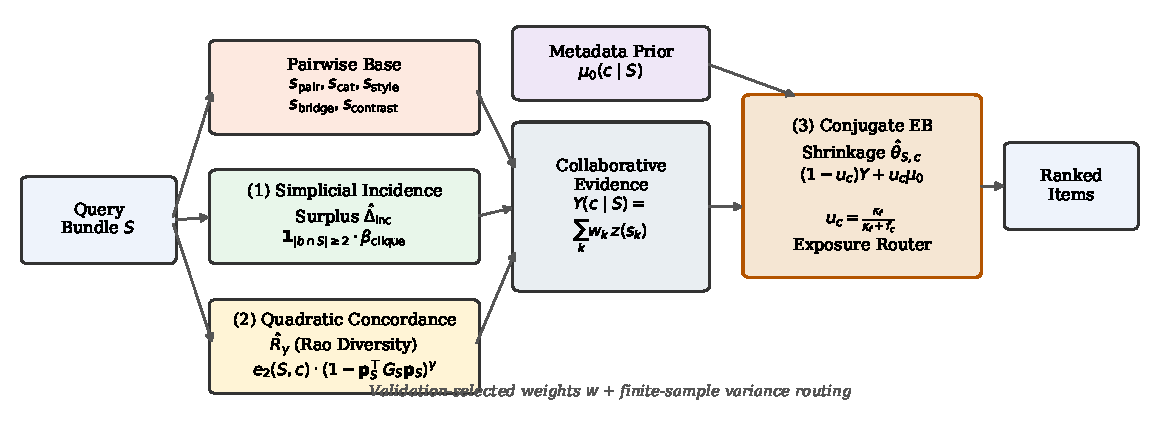
\includegraphics[width=\linewidth]{figs/fig_framework.pdf}
  \caption{Overview of \textsc{BundleFuse}. Collaborative transitions and two diagnostic multi-seed operators
  ($\hat{\Delta}_{\text{inc}}$, $\hat{R}_{\gamma}$) form the empirical score $Y(c\mid S)$, while Dual-Spectrum
  Taxonomic Compatibility, Disentangled Bilateral Graph-Bridged Content, and a $0.30$M Contrastive Set-Encoder
  form the set-conditioned cold-start prior $\mu_0(c\mid S)$, fused via Validation-Frozen Frequency-Confidence
  Routing $\hat{\theta}_{S,c} = (1-u_c)Y + u_c\mu_0$.}
  \label{fig:framework}
\end{figure}

\subsection{Problem Formulation and Collaborative Base}
\label{sec:prob}
\label{sec:features}
Let $\mathcal{I}$ ($|\mathcal{I}|=n$) be the item catalogue and $\mathcal{B}_{\text{train}}$ the training bundles
with incidence matrix $B\in\{0,1\}^{|\mathcal{B}_{\text{train}}|\times n}$, item frequencies
$f_i = \sum_{b} B_{b,i}$, and bundle sizes $|b| = \sum_i B_{b,i}$. Given a partial query bundle $S \subset b$,
the goal is to rank all candidates $c \in \mathcal{I}\setminus S$ to recover $b\setminus S$.

On warm items ($f_c > 0$), first-order collaborative transitions use the 1-skeleton projection
$C = B^{\!\top}B - \operatorname{diag}$, degree-normalised pairwise transitions
$W_{\text{pair}} = B^{\!\top}\operatorname{diag}\big((|b|+1)^{-\gamma_{\text{vol}}}\big)B\operatorname{diag}\big((f+\alpha_0)^{-\alpha_{\text{deg}}}\big)$
($\operatorname{diag}(W_{\text{pair}})=0$), and two-hop smoothing via the exact zero-diagonal \emph{row-stochastic}
bipartite walk $P_{\text{rw}} = D_{\text{row}}^{-1}(D_I^{-1}B^{\!\top}D_B^{-1}B - \operatorname{diag})$ or its
symmetrically normalised counterpart $\mathcal{P}$:
\begin{equation}
  s_{\text{pair}}(c\mid S) = \sum_{s\in S} (W_{\text{pair}})_{c,s}, \qquad
  s_{\text{diff2}}(c\mid S) = \big(\mathcal{P}\,s_{\text{pair}}(\cdot\mid S)\big)_c.
  \label{eq:pair}
\end{equation}
When user or session IDs are observed on training bundles, user/session co-occurrence matrices $C_u, C_s$ (and
per-user within-basket loyalty on retail) enter additively alongside~\eqref{eq:pair}. However, for any unexposed
cold item ($f_c = 0$), every collaborative channel in~\eqref{eq:pair} is identically zero (producing a negative
catalogue $z$-score after column standardisation).

\subsection{Pillar I: Dual-Spectrum Taxonomic \& Slot-Exclusion Prior}
\label{sec:ontology-method}
A central failure mode of standard content/category priors in bundle completion is conflating \emph{off-diagonal
complementarity} (e.g., shirt $\leftrightarrow$ trousers) with \emph{on-diagonal slot duplication} (e.g., recommending
a second shirt when $S$ already contains a shirt). Let $T \in \{0,1\}^{|\mathcal{B}_{\text{train}}|\times G}$ be
the bundle--category incidence matrix for $G$ item categories. \texttt{DualSpectrumOntology} separates three
distinct taxonomic signals from $T$ (fitted strictly on $\mathcal{B}_{\text{train}}$):
\begin{enumerate}\itemsep1pt
  \item \textbf{Off-diagonal complementarity PMI ($P_{\text{cat}}$):} Setting $\operatorname{diag}(T^{\!\top}T)=0$,
  positive pointwise mutual information $(P_{\text{cat}})_{g,g'} = \max\!\big(0, \log\frac{(T^{\!\top}T)_{g,g'}
  \sum T}{\sum_b T_{b,g}\sum_b T_{b,g'}}\big)$ captures cross-category slot affinity.
  \item \textbf{Signed on-diagonal slot-saturation penalty ($s_{\text{slot}}$):} For each category $g$, let
  $\hat{\delta}_g = \frac{\#\{b : \sum_{i\in b}\mathbf{1}[\text{cat}(i)=g] \ge 2\} + 0.5}{\#\{b : \sum_{i\in b}\mathbf{1}[\text{cat}(i)=g] \ge 1\} + 1}$
  be its empirical intra-bundle duplication rate. Whenever $\hat{\delta}_{\text{cat}(s)} < \tau_{\text{dup}}$
  ($0.15$), candidates sharing seed $s$'s category receive a signed self-exclusion penalty:
  \begin{equation}
    s_{\text{slot}}(c\mid S) = -\sum_{s\in S : \hat{\delta}_{\text{cat}(s)} < \tau_{\text{dup}}}
    \mathbf{1}\big[\text{cat}(c) = \text{cat}(s)\big]\big(1 - \hat{\delta}_{\text{cat}(s)}\big).
    \label{eq:slot}
  \end{equation}
  \item \textbf{Soft fuzzy sub-type complementarity ($M_{\text{soft}}P_s$) and homophily ($P_{\text{homo}}$):}
  Because coarse catalogue categories merge distinct functional sub-types (e.g., dress shoes vs.\ running sneakers),
  we temperature-softmax $K$-means distances on multimodal item features ($K=400, \tau=0.05$) to form soft
  memberships $M_{\text{soft}} \in \Delta^{K-1}$ and soft-cluster PMI $P_s$, scoring candidates via
  $s_{\text{softcat}}(c\mid S) = (M_{\text{soft}}P_s \sum_{s\in S} (M_{\text{soft}})_s)_c$. Conversely, in
  similarity-driven domains (music playlists), on-diagonal artist/album inverse-degree incidence $P_{\text{homo}}$
  captures cohesive artist/album continuation.
\end{enumerate}

\subsection{Pillar II: Disentangled Bilateral Content Bridge \& Contrastive Set-Encoder}
\label{sec:bridge-method}
\label{sec:reasoner}
Raw text/visual embeddings $x_i \in \mathbb{R}^d$ are dominated by category-level semantics, which are redundant
with Pillar I and misleading when complementary items come from different categories.
\texttt{BilateralContentBridge} first removes category centroids to isolate within-category \emph{style}:
\begin{equation}
  \tilde{x}_i = \frac{x_i - \bar{x}_{\text{cat}(i)}}{\lVert x_i - \bar{x}_{\text{cat}(i)}\rVert_2 + \epsilon},
  \qquad \bar{x}_g = \frac{1}{|I_g|}\sum_{j\in I_g} x_j.
  \label{eq:disentangle}
\end{equation}
Second, to bridge the cold--warm divide, we diffuse $\tilde{x}$ across the zero-diagonal bipartite bundle operator
$\mathcal{P}$ to obtain bilateral graph-bridged representations $\tilde{b}_i = \operatorname{norm}\big(\tilde{x}_i
+ \alpha_{\text{bridge}}\mathcal{P}(\tilde{x})_i\big)$. Even when candidate $c$ is cold ($f_c=0 \implies
\mathcal{P}(\tilde{x})_c = 0$), its inner product $\tilde{b}_c^{\!\top}\tilde{b}_s = \tilde{x}_c^{\!\top}\big(\tilde{x}_s
+ \alpha_{\text{bridge}}\mathcal{P}(\tilde{x})_s\big)$ matches $c$'s raw style directly against the \emph{collaborative
neighborhood style} of warm seed $s$. Alongside $\tilde{x}$ and $\tilde{b}$, a lightweight two-layer MLP
$\phi_\theta:\mathbb{R}^d\to\mathbb{R}^h$ ($h=128, \le 0.30\text{M}$ parameters) pools seed representations via
learned attention $r(S) = \sum_{s\in S}\alpha_s \phi_\theta(x_s)$ and is trained with InfoNCE~\cite{infonce} against
popularity$^{0.75}$-sampled negatives.

\subsection{Diagnostic Higher-Order Operators: $\hat{\Delta}_{\text{inc}}$ and $\hat{R}_{\gamma}$}
\label{sec:incidence}
\label{sec:concordance}
To test whether explicit $(k\ge 3)$-way hypergraph co-occurrence or second-order seed agreement improves over
Pillars I--II, we isolate two closed-form higher-order operators:
\begin{enumerate}\itemsep1pt
  \item \textbf{Simplicial Hyperedge Incidence Surplus ($\hat{\Delta}_{\text{inc}}$):} Following studies of
  simplicial closure and clique-expansion loss~\cite{benson2018,ebli2020,prokopchik2022,lee2024}, we isolate pure
  $(k\ge 3)$-way joint bundle co-occurrence from~\eqref{eq:pair} via
  \begin{equation}
    \hat{\Delta}_{\text{inc}}(c\mid S)
    = \sum_{b \in \mathcal{B}_{\text{train}} : c \in b}
      (|b|+1)^{-\gamma_{\text{vol}}}
      \Big(\sum_{s\in b\cap S}(f_s+\alpha_0)^{-\alpha_{\text{deg}}}\Big)\,
      \beta_{\text{clique}}\max\!\big(0,\,|b\cap S|-1\big).
    \label{eq:incidence}
  \end{equation}
  Equation~\eqref{eq:incidence} is strictly positive if and only if a training bundle contains $c$ together with at
  least two seeds from $S$ ($\Pr(\exists b : |b\cap S|\ge 2)$).
  \item \textbf{Redundancy-Corrected Quadratic Concordance ($\hat{R}_{\gamma}$):} Using the $O(|S|)$ Newton identity
  $2e_2(w) = (\sum_{s\in S} w_{c,s})^2 - \sum_{s\in S} w_{c,s}^2$ from Factorization
  Machines~\cite{rendle2010,blondel2016} with total support $A_c = \sum_{s\in S} w_{c,s}$ and shares
  $p_{c,s} = w_{c,s}/A_c$, and weighting seed pairs by Rao's quadratic diversity~\cite{rao1982} over seed
  similarity $G_S \in [0,1]^{|S|\times|S|}$ gives degree-1 homogeneous concordance:
  \begin{equation}
    \hat{R}_{\gamma}(c\mid S;\tau)
    = \frac{A_c^2}{A_c + \tau} \sum_{s\neq s'\in S} K_S(s,s';\gamma)\,p_{c,s}\,p_{c,s'},
    \qquad K_S(s,s';-1) = 1 - G_{s,s'}.
    \label{eq:rao}
  \end{equation}
\end{enumerate}
As we show in \S\ref{sec:control}, isolating $\hat{\Delta}_{\text{inc}}$ and $\hat{R}_{\gamma}$ yields a crisp
diagnostic finding: once Pillars I and II are present, $\hat{\Delta}_{\text{inc}}$ and $\hat{R}_{\gamma}$ add only
$+0.00$ to $+0.34$\,pp overall, proving that cold-start prior construction and exposure routing---not higher-order
collaborative algebra---drive performance.

\subsection{Pillar III: Validation-Frozen Frequency-Confidence Routing}
\label{sec:eb}
\label{sec:fusion}
\label{sec:complexity}
Let $Y(c\mid S)$ denote the fused score across all active channels and let $s_{\text{prior}}(c\mid S)$ denote the
set-conditioned prior built from Pillars I--II (taxonomic, bridged-content, and contrastive channels, which require
zero collaborative exposure for candidate $c$). Because $Y(c\mid S)$ penalises unexposed items ($f_c=0$) with
negative collaborative $z$-scores, we route between $Y(c\mid S)$ and the variance-matched prior
$\mu_0(c\mid S) = \gamma_{\text{val}} s_{\text{prior}}(c\mid S)$ via inverse-frequency confidence
weights~\cite{bell2007,agarwal2009}:
\begin{equation}
  \hat{\theta}_{S,c}
  = (1 - u_c)\,Y(c\mid S) + u_c\,\mu_0(c\mid S),
  \qquad u_c = \frac{\kappa_f}{f_c + \kappa_f}, \quad
  \gamma_{\text{val}} = \frac{\sigma_{\text{val}}(Y)}{\sigma_{\text{val}}(s_{\text{prior}}) + \epsilon}.
  \label{eq:posterior}
\end{equation}
Freezing the scalar $\gamma_{\text{val}}$ on the validation split guarantees that test-time predictions are
\emph{strictly invariant to test batch composition} ($0.000000$ cross-query drift, verified in
\texttt{tests/test\_audit.py}). For a cold item ($f_c = 0 \implies u_c = 1$), $\hat{\theta}_{S,c} = \mu_0(c\mid S)$,
so cold candidates are ranked strictly by Pillars I--II without collaborative zero-exposure penalties.

\paragraph{Why homoscedastic Empirical-Bayes moment-matching fails on sparse bundles, and why $\kappa_f$ is validation-tuned (or fixed).}
Under an idealized homoscedastic Normal--Normal model ($\theta_{S,c}\mid\mu_0 \sim \mathcal{N}(\mu_0,\sigma_0^2)$,
$Y\mid\theta_{S,c},f_c \sim \mathcal{N}(\theta_{S,c}, \sigma_\epsilon^2/f_c)$), the posterior mean takes the
form~\eqref{eq:posterior} with $\kappa_f = \sigma_\epsilon^2/\sigma_0^2$, and regressing $v_c = \mathbb{E}_S[(Y -
\mu_0)^2]$ on $1/f_c$ across warm items ($f_c > 0, \operatorname{Var}(1/f_c)>0$) should yield positive slope
$\tilde{\sigma}_\epsilon^2 > 0$. We retain this OLS check in \texttt{fit\_variance\_components} as a diagnostic test
and show in Table~\ref{tab:exposure_buckets} that \emph{real bundle data rejects the homoscedastic noise assumption on
$7$ of $8$ datasets} ($\tilde{\sigma}_\epsilon^2 < 0$): rare items ($f_c=1$) are heavily zero-inflated across queries
(near-zero dispersion across $S$), whereas popular hubs ($f_c \gg 1$) co-occur across diverse queries (large
dispersion across $S$). Rather than treating the Gaussian derivation as load-bearing when its moment estimator clips
to the floor ($0.05$), we treat~\eqref{eq:posterior} directly as \textbf{frequency-confidence backoff} where $\kappa_f$
is either (i)~selected on the validation split from a 5-point grid $\{0.0, 0.05, 0.1, 0.5, 1.0, 5.0\}$, or
(ii)~held at a single universal value $\kappa_f = 0.5$ across all datasets (\S\ref{sec:control}, Table~\ref{tab:tuning}).
